\documentclass[conference]{IEEEtran}

% \hyphenation{op-tical net-works semi-conduc-tor}


\ifCLASSINFOpdf
  \usepackage[pdftex]{graphicx}
  % declare the path(s) where your graphic files are
  \graphicspath{{../pdf/}{../jpeg/}}
  % and their extensions so you won't have to specify these with
  % every instance of \includegraphics
  \DeclareGraphicsExtensions{.pdf,.jpeg,.png}
\else
  % or other class option (dvipsone, dvipdf, if not using dvips). graphicx
  % will default to the driver specified in the system graphics.cfg if no
  % driver is specified.
  \usepackage[dvips]{graphicx}
  % declare the path(s) where your graphic files are
  \graphicspath{{../eps/}}
  % and their extensions so you won't have to specify these with
  % every instance of \includegraphics
  \DeclareGraphicsExtensions{.eps}
\fi

\usepackage[export]{adjustbox}
\usepackage{color}
\usepackage{breqn}
\usepackage[linesnumbered,ruled]{algorithm2e}

\newcommand{\sys}{{\sc GeoGig}}

% to remove
\newcommand{\framework}{{\sc GeoHighlight}}
\newcommand{\pb}{{\sc GeoGuide}}
\newtheorem{example}{Example}
\newtheorem{problem}{Problem}
\newtheorem{definition}{Definition}

\begin{document}

%\title{GeoHighlight: Interactive Guidance-based Visualization for Spatiotemporal Data}
\title{GeoGIG: A Guidance-based Visualization Framework for Spatiotemporal Data}


% author names and affiliations
% use a multiple column layout for up to three different
% affiliations
\author{\IEEEauthorblockN{Behrooz Omidvar-Tehrani}
\IEEEauthorblockA{Department of Computer Science\\
The Ohio State University\\
{\em omidvar-tehrani.1@osu.edu}}
\and
\IEEEauthorblockN{Pl\'acido A. Souza Neto, Gustavo Guerino}
\IEEEauthorblockA{Federal Institute of Rio Grande do Norte\\
IFRN, Brazil\\
{\em placido.neto@ifrn.edu.br, gustavo.guerino@academico.ifrn.edu.br}}
}

% make the title area
\maketitle


\begin{abstract}
Spatiotemporal data is becoming increasingly available in various domains such as transportation and social science. There exists huge potentials to discover patterns and trends in this data for better decision making. A visualization suite provides visual interpretations of this data. However there exist three principled challenges which are not perfectly addressed in current visualization tools: $i.$  the tool should be ``generic'' enough to provide insights for any spatiotemporal data; $ii.$ it should be ``interactive'' to facilitate sub-second analyst-tool loops; $iii.$ it should be able to ``guide'' analysts in an exploratory analysis scenario through potential interesting directions. In this paper, we introduce \sys, an interactive guidance-based visualization framework for spatiotemporal data. We discuss the functionality of \sys\ and provide two scenarios that illustrate the usability of \sys\ on different spatiotemporal datasets.
\end{abstract}

\IEEEpeerreviewmaketitle

\vspace{-5pt}
\section{Introduction} 
Nowadays, there exists huge amounts of spatiotemporal data in various fields of science. Understanding patterns and trends through visualizing spatiotemporal data improves decision making. Some instance applications of spatiotemporal data analysis are smart city management and autonomous transport. Traditionally, an exploratory analysis scenario begins by preparing the data and employing a data visualization product like Tableau\footnote{\it http://www.tableau.com} or Spotfire\footnote{\it http://spotfire.tibco.com} to explore a subset of data. However, with the growing size of spatiotemporal datasets, this classical analysis approach is not practical anymore. We recognize following challenges in visualizing spatiotemporal data.

  \begin{figure}
   \centering
   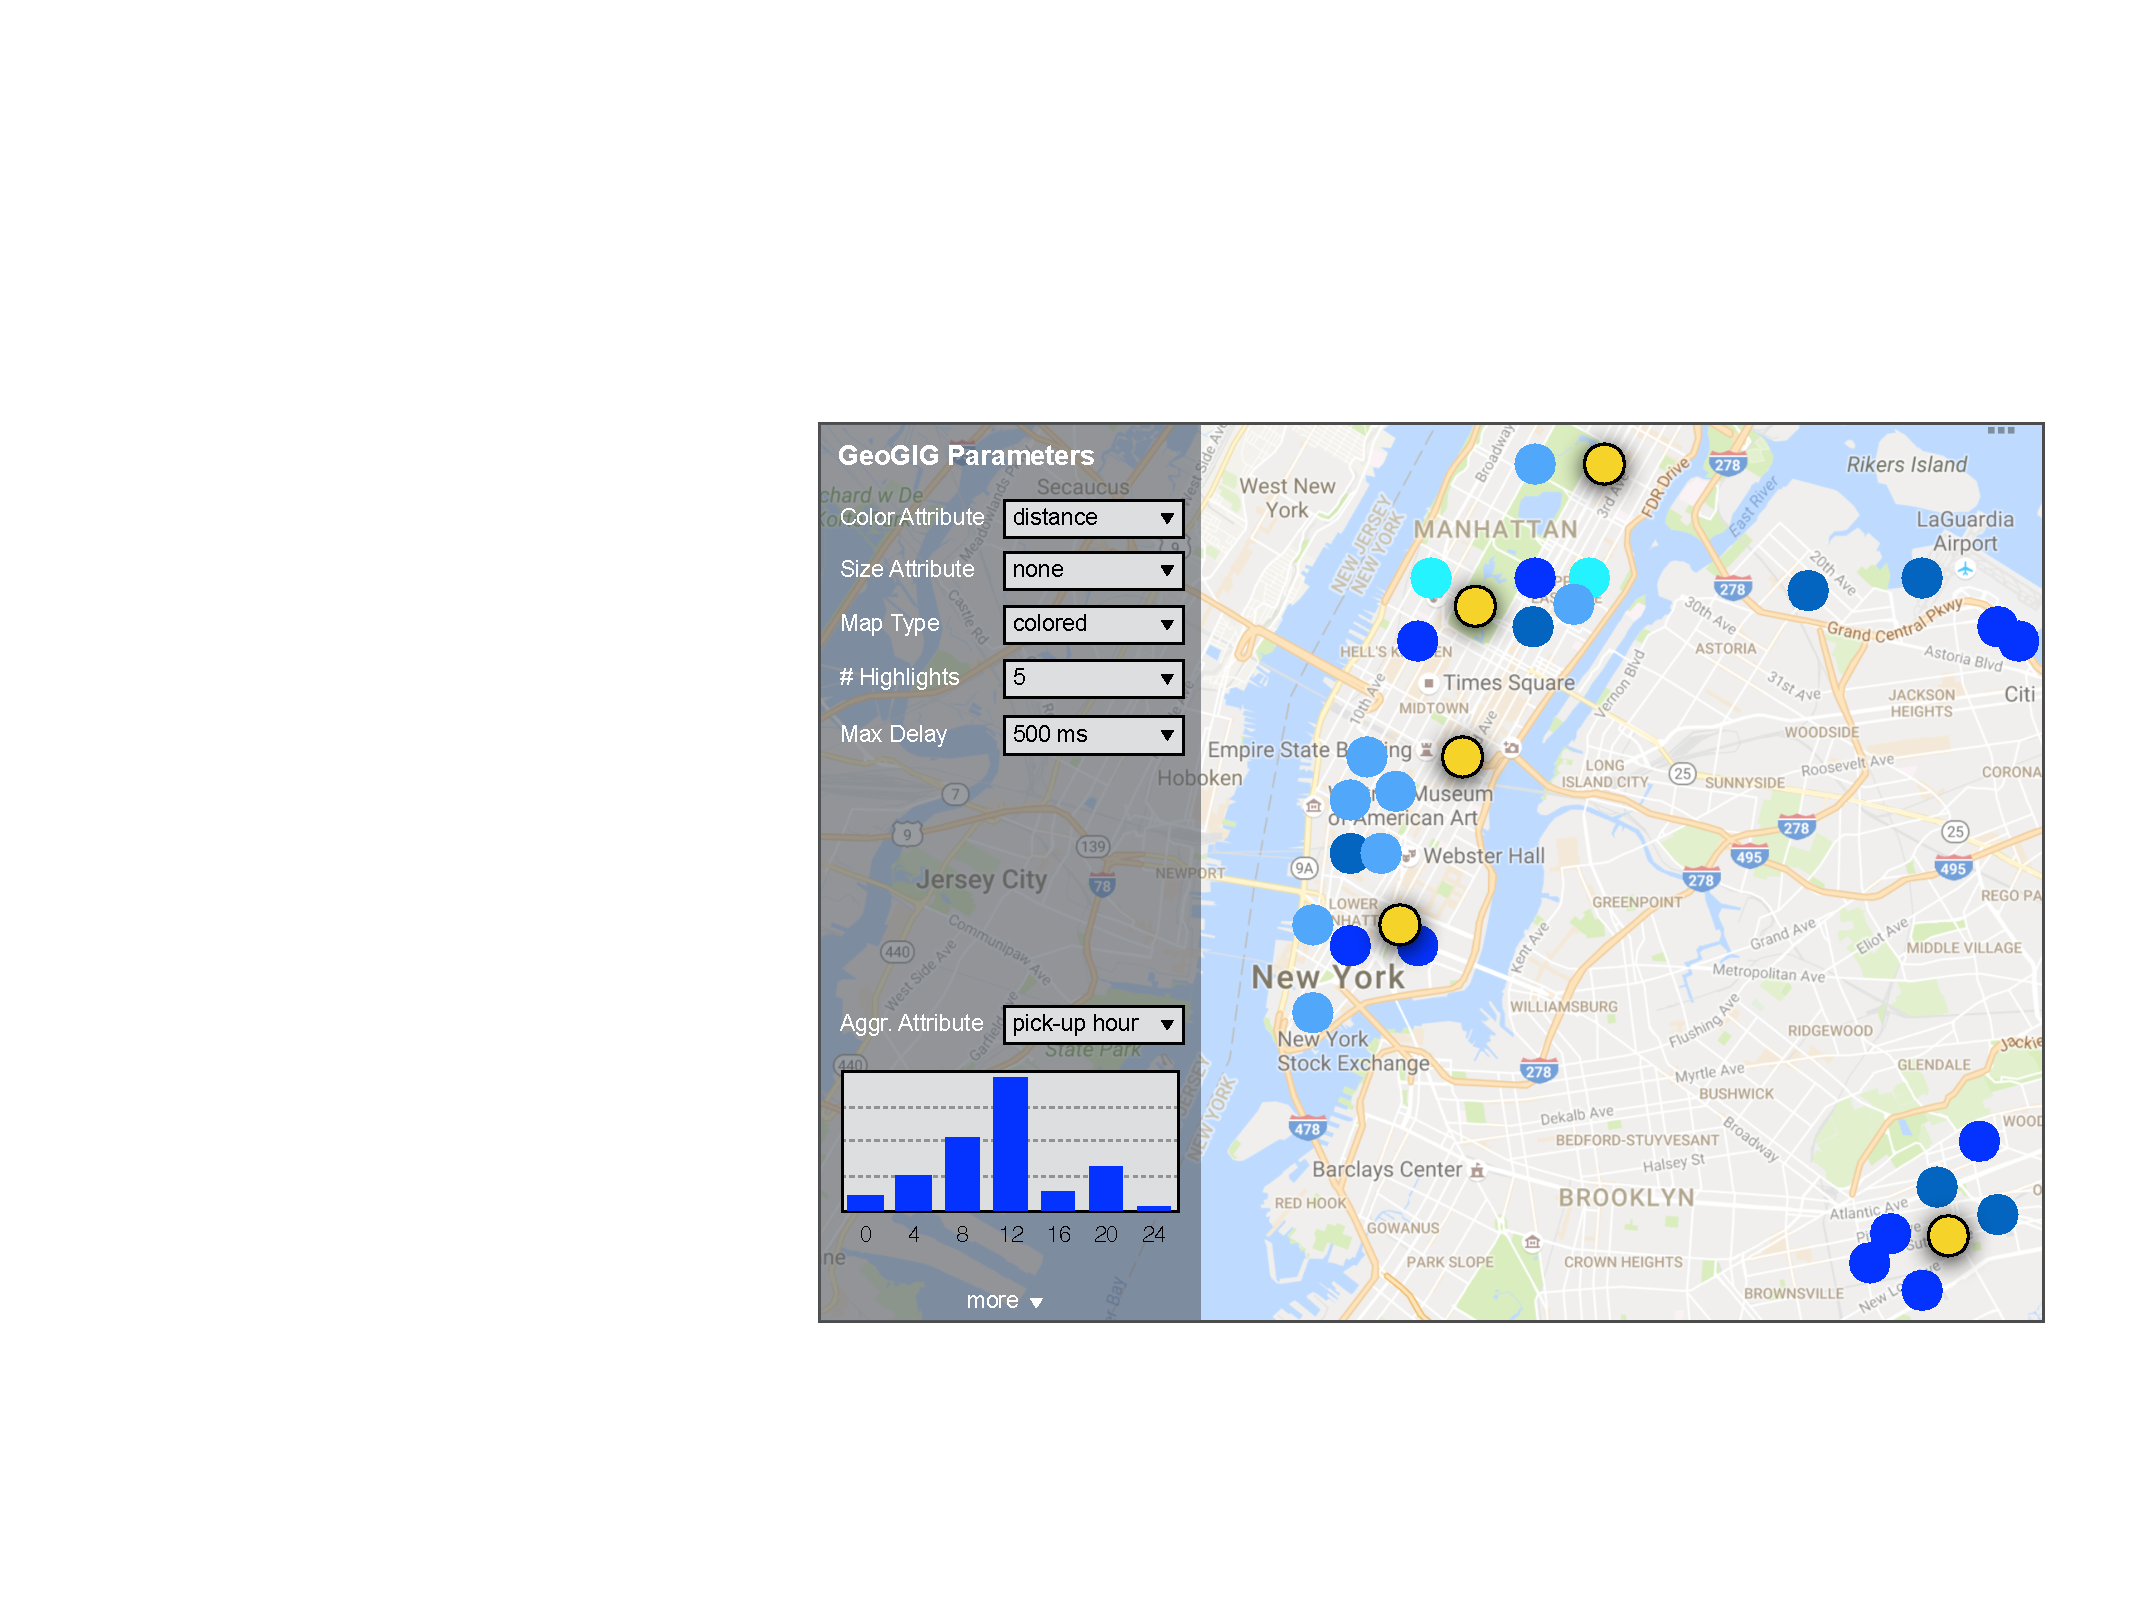
\includegraphics[width=\columnwidth]{figs/dashboard}
 \caption{\small \sys\ depicts few New York taxi drop-off points. Five points are highlighted by the guidance component. Pick-up hour is selected as the aggregated attribute.}
 \label{fig:dashboard}
 \vspace{-15pt}
 \end{figure}

%To overcome this challenge, visualization environments offer a plethora of operations to manipulate data (filter, aggregate, etc.). In practice, this duplicates the problem: the analyst is left alone in a huge space of data and operations. In an exploratory context, the principled challenge for the analyst is {\em ``what to see next''} during the analysis process. A {\em guidance mechanism} is necessary to point out potential future directions of analysis.

\noindent {\bf Genericness.} Most visualization suites do not generalize to different types of data. This is a critical challenge in spatiotemporal context due to its huge diversity from transportation data to geo-political and geo-health data. Although tools like {\sc D3}\footnote{\it https://d3js.org} and {\sc Vega} \cite{satyanarayan2016reactive} introduce grammars for generic visualization, formalizing a problem in form of a grammar needs some expertise which an analyst may not have.

\noindent {\bf Interactivity.} The main focus of current approaches is to generate a single-shot visualization. However, in most analysis scenarios, there is a need to interact with the tool by manipulating data (filter, aggregate, etc.) Due to the gigantic size of the data and inefficient infrastructure, the interaction usually takes up to minutes and impose unnecessary waiting time on the analyst. Hence there is a need for a visualization tool to be interactive.

\noindent {\bf Guidance.} Even in an interactive visualization tool, another critical challenge is that often analysts are lost in the huge amount of visualized points and cannot easily decide ``what to see next''. Hence a guidance approach is necessary in order to automatically highlight few directions for further investigations.

To tackle the aforementioned challenges, we propose \sys, i.e., a generic, interactive and guidance-based approach for spatiotemporal data. \sys\ helps analysts to load and visualize their spatiotemporal data of any type without following any complicated grammar. Then the analyst observes patterns and trends from different parts of data interactively. Also, \sys\ provides recommendations in each interactive step to guide the analyst through potential interesting directions.

% We inspire from both recommendation \cite{Omidvar-Tehrani:2015} and visual highlighting \cite{Liang2010,Robinson2011} methodologies and propose \sys\ as a solution to aforementioned challenges. \sys\ is a visualization framework for spatiotemporal data which guides the analyst throughout the process towards interesting points. In this paper, we propose this guidance approach for analysis of huge datasets with geographic informations. So, the analyst considers the guidance and picks a direction for the next analysis iteration.

%Given a geographical point of interest, the question is then how to recommend other points to be considered in future analysis steps in form of guidance. In this paper, we focus on one specific guidance approach, i.e., highlighting $k$-best points given a point of interest. Those $k$ points should have high quality. Quality is formulated as optimization of two dimensions: {\em relevance} and {\em diversity}. Optimizing relevance ensures that recommended points are in-line with what the analyst has already liked. Optimizing diversity results points which are as different as possible from each other and unveil different aspects of analysis. 

\vspace{-5pt}
\section{Framework}
\sys\ employs various components and strategies to tackle the challenges of genericness, interactivity and guidance. The aim of the proposed application is to $i.$ enable analysts visualize any spatiotemporal data with the least burden, $ii.$ interact with the data in sub-seconds and $iii.$ receive recommendations during the analysis process for further investigations.

\sys\ is designed as a web service and runs in a browser. Figure \ref{fig:dashboard} illustrates a screen-shot of \sys\ on New York taxi dataset. To initialize the analysis, the analyst needs to drag-and-drop her dataset (in form a CSV file) into the browser. \sys\ exploits {\sc WebTables} \cite{cafarella2008webtables} to find the best matching schema for the input dataset. \sys\ performs the following execution command to visualize the dataset:

\noindent {\tt \small geogig ds=name [param=val]$^*$ [udf: param=val]$^*$;}

The only required parameter for \sys\ is the dataset {\tt \small name} which is given by the drag-and-drop. A set of visualization settings in form of {\tt \small [param=val]} customizes the visualization. 
% Each parameter {\tt param} has a default value which will be applied if no value is provided by the analyst.
For instance in Figure \ref{fig:dashboard}, {\tt \small color=distance}, hence drop-off points are colored darker if they belong to longer trips. Interestingly, points closer to airports are often darker as often longer trips are need rich airports.

\sys\ supports the integration of spatiotemporal User-Defined Functions (i.e., {\tt \small [udf: param=val]} in the execution commands) to satisfy specific needs of analysts. For instance, an analyst may create a UDF to color points in red if their tip amount is higher than \$4.

\sys\ recognizes three sets of attributes: {\em principle}, {\em aggregation} and {\em peripheral}. The {\em principle set} contains attributes which are necessary to visualize data on a geographical map, i.e., latitude and longitude. Altitude can also be considered in case of 3D projection (e.g., aviation data analysis). If \sys\ fails to automatically complete the principle set, it will ask the analyst to manually mark those attributes. The {\em aggregation set} contains ordinal attributes which can be aggregated to provide complementary insights on visualized points, e.g., time-of-day, week day, etc. In Figure \ref{fig:dashboard}, ``pick-up hour'' is selected as the aggregated attribute and the abundance of points in 24 hours is shown in a histogram. Last, the remaining set of attributes is called {\em peripheral}. Hovering each point on the map will pop-up the list of peripheral attributes for that particular point.

A histogram exhibits aggregated counts for an attribute of choice from the set of aggregation attributes. \sys\ exploits Crossfilter charts \cite{cf} as the histogram which enables {\em coordinated views}, i.e., a brush on the histogram will immediately update the map. Normally this task needs a query execution per brush, which is time-consuming. By exploiting the notion of {\em incremental queries}, the task evolves to sub-second execution.

\sys\ scans the input dataset only once. For further analysis steps, it employs a {\em caching} strategy so that it doesn't require a connection to the dataset more than once and all other filters and brushes will be done online without re-querying. We also consider a {\em sampling} strategy to deliver visualizations in sub-seconds independent from the query result size. The combination of caching and sampling mechanisms assures that all analyst's requests can be served without delay independent from the nature of the request. This enables interactive analysis of spatiotemporal data.

At each step of the interactive process, a guidance component recommends a limited set of points which are potentially interesting for the analyst for further investigation. The guidance component is an adaptation from our previous work~\cite{Omidvar-Tehrani:2015} to the spatiotemporal context. Figure \ref{fig:dashboard} illustrates recommended points in yellow. Intuitively, the guidance component returns $k$ points which are {\em highly relevant} to previous analyst's choices. Those $k$ points are also {\em highly diverse} to cover the analysis space so that the analyst can investigate on different aspects of data. The guidance component is an optimization algorithm which aims to maximize relevance and diversity. However, to respect interactivity, a time limit will be given so that the algorithm performs a best-effort strategy up to the limit. The value of time limit and the size constraint ($k$) can be set in the setting bar (Figure \ref{fig:dashboard} left).

\vspace{-5pt}
\section{Demonstration}

\noindent {\bf Data.} We illustrate the functionality of \sys\ in form of realistic scenarios on New York taxi\footnote{\it https://data.cityofnewyork.us/view/gn7m-em8n} and New York bike\footnote{\it https://s3.amazonaws.com/tripdata/index.html} datasets. We chose those datasets because they are publicly available and frequently exploited in spatiotemporal research (e.g., in \cite{DBLP:journals/debu/FreireCVZ16}). However, particpants can bring their own spatiotemporal datasets in form of a CSV file to apply to \sys.

\noindent {\bf Implementation.} The \sys\ engine is implemented in Python 2.7.10 and the graphical user interface is based on Node.js. The visualization components are implemented using {\sc D3}\footnote{\it https://d3js.org} and the geographical map is based on {\sc Google Maps API}\footnote{\it https://developers.google.com/maps/}. The demo is fully client-side and on-the-browser which makes it platform-independent. 

\noindent {\bf Scenario 1.} We employ New York taxi dataset for this scenario. The  dataset contains 173,179,759 records of taxi trips and 18 attributes such as pickup and dropoff date/time, passenger count, tip amount and trip distance. Consider Lucas, a data scientist who is tasked to optimize New York taxi trips. Focusing on cab-idle locations, he wants to discover which neighborhoods work the best for which drivers to increase the overall availability. Lucas employs \sys\ and follows a case-by-case inspection as his analysis methodology. We show how Lucas benefits from the guidance component to discover relevant points to his interests. We also show that he observes different aspects of data without delay due to interactivity considerations.

\noindent {\bf Scenario 2.} We employ New York bike dataset for this scenario. The New York bike dataset contains bike trips from 2013 to 2016, and 15 attributes such as start/end station, trip duration and distance. Consider Stella, a data scientist who is tasked to optimize New York bike station locations in New York by analyzing bike historical data. We show how guidance component helps Stella to recognize locations with similar profile in diverse locations. Also, we show that she can focus on different parts of data (e.g., male and female riders) to make use-case studies interactively.


 % \begin{figure}[!ht]
 %   \centering
 %   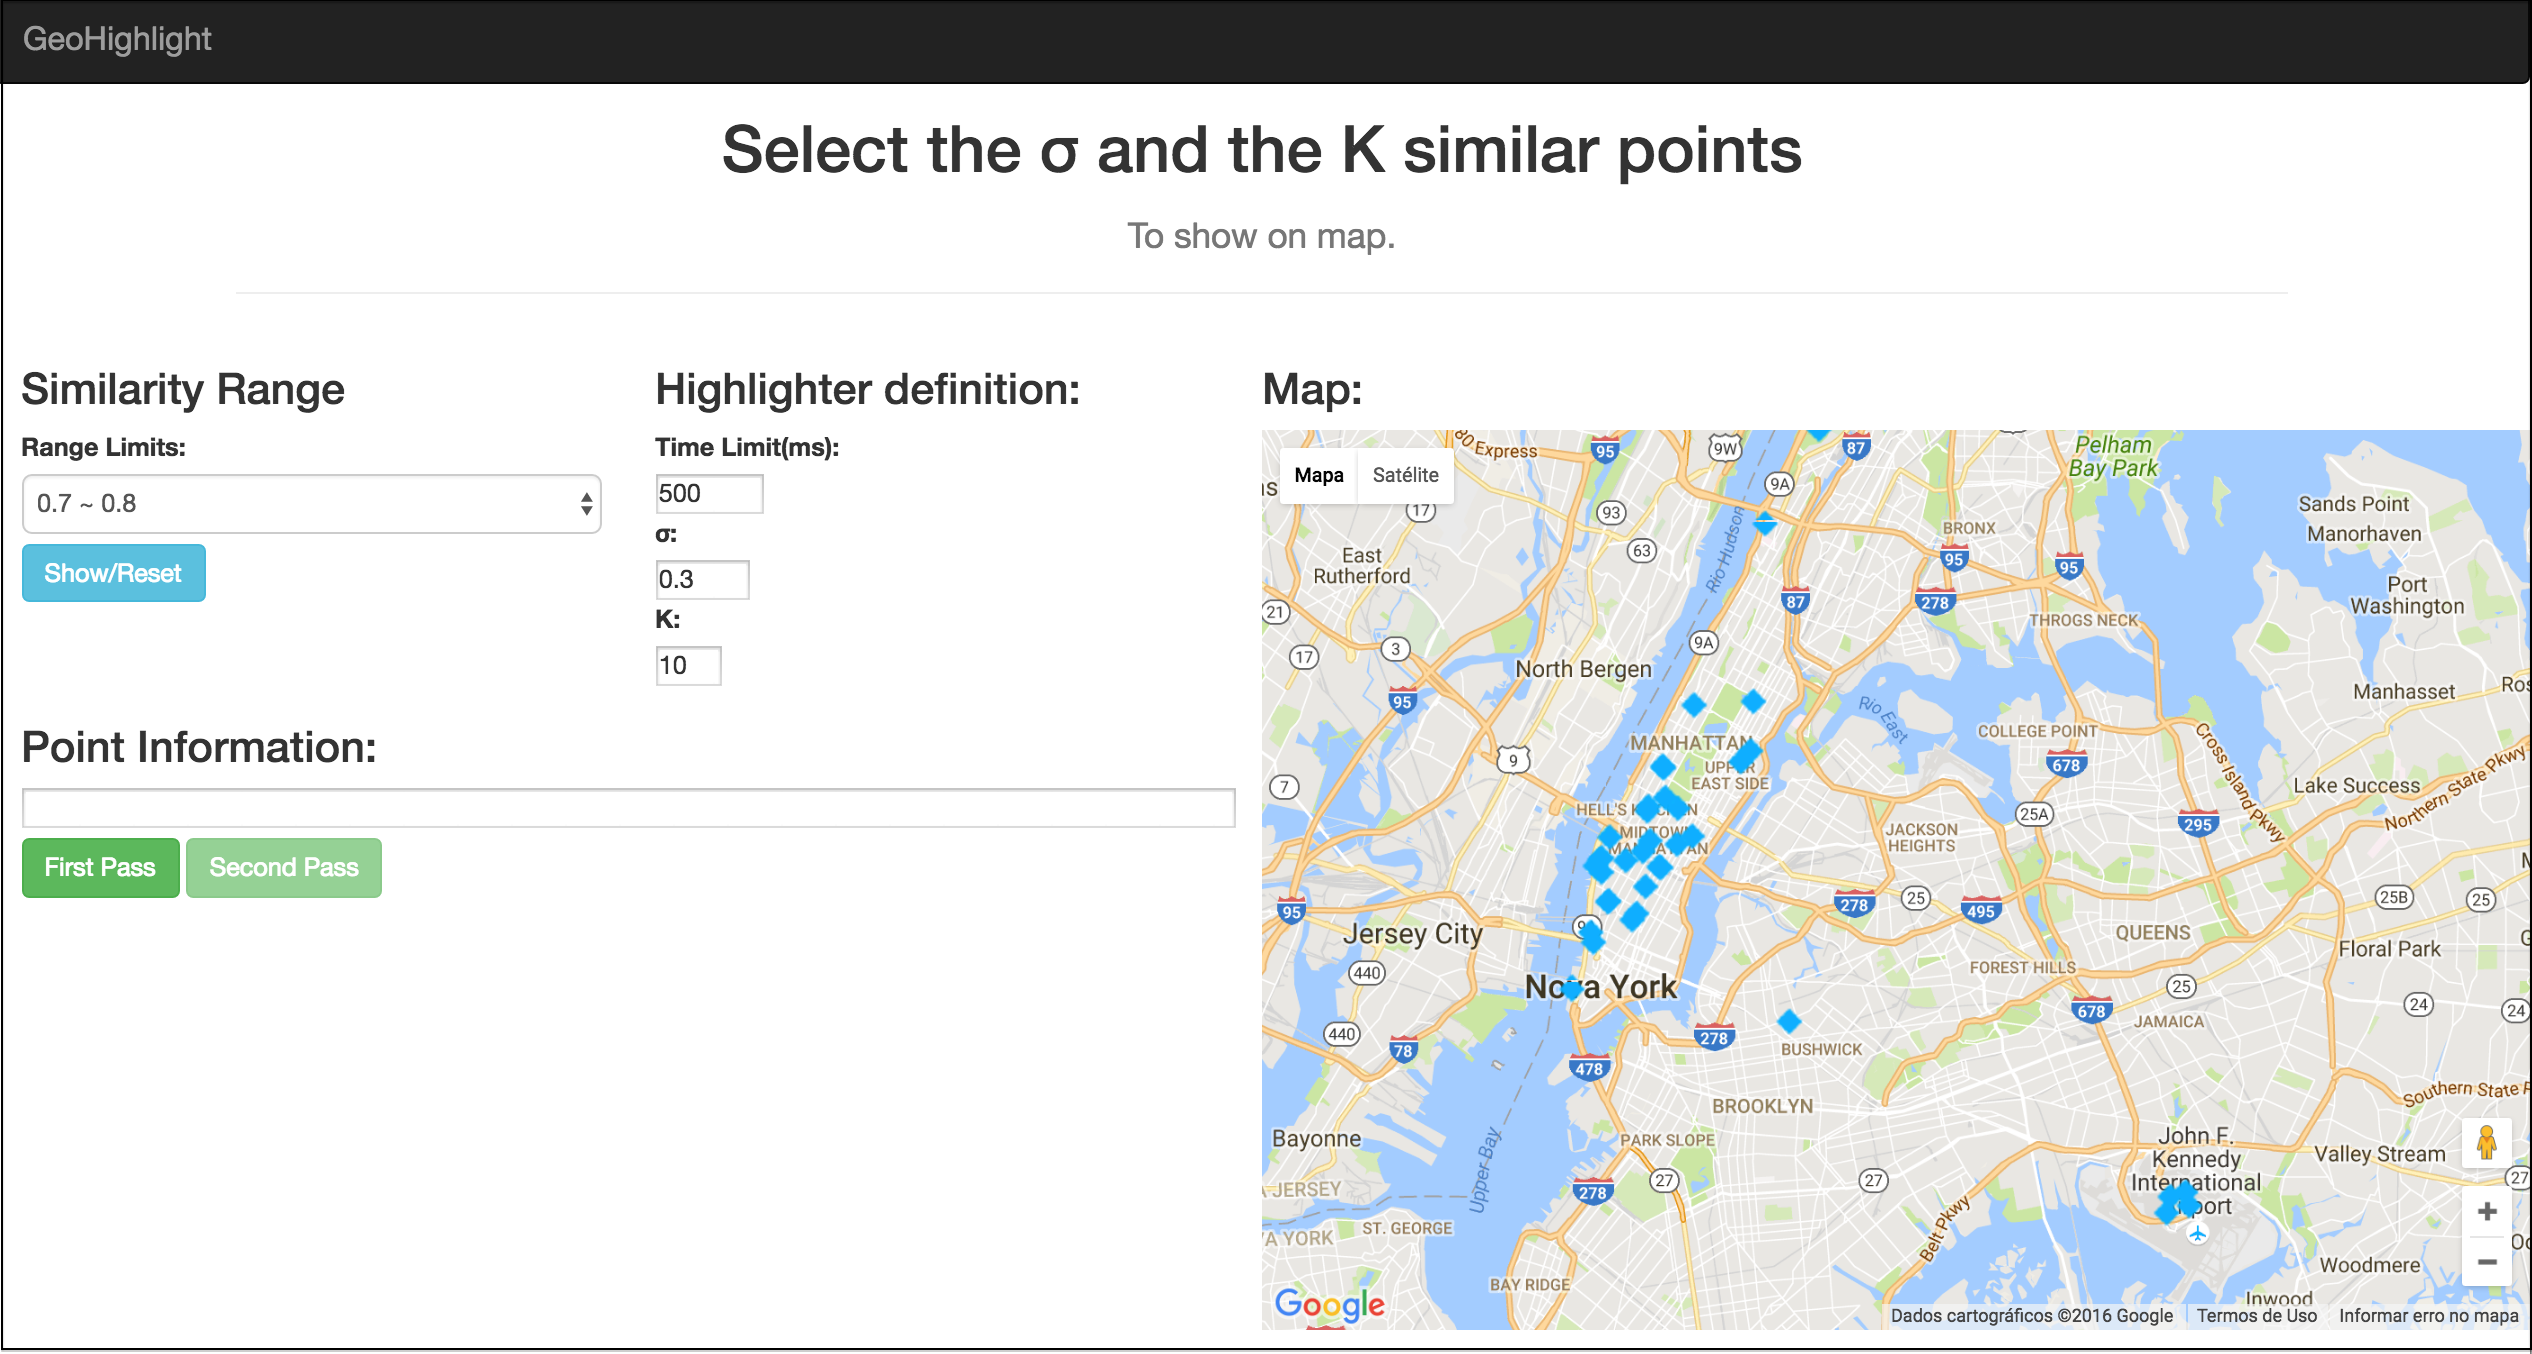
\includegraphics[width=\columnwidth, frame]{figs/dashboard1}
 % \caption{\framework\ Dashboard [New York Taxi Scenario] - View of a set of taxi pick-up and drop-off points.}
 % \label{fig:dashboard}
 % \vspace{-10pt}
 % \end{figure}


 
 

 
%  \section{Conclusion}
 
%  In this demo we have presented \sys, a generic and interactive
% framework for visualization of spatiotemporal data. Some future extensions include the integration
% of generic query approach based on \cite{VartakRMPP15}, and we also want to consider an analyst profile vector which is built during interactive steps and will be exploited to return more analyst-tailored results.

\vspace{-5pt}
\bibliographystyle{abbrv}
\bibliography{main}




% that's all folks
\end{document}


